%continuing the part of Berendsen thermostat


As we have seen, the Berendsen algorithm is a smooth, continuous version of the velocity rescaling. In order to implement it, we take the velocity rescaling algorithm: 

 \begin{algorithm}[H]\label{velocity_rescaling}
			\caption{Velocity rescaling algorithm}
			\begin{algorithmic}[1]
				\For{$i=1,...,nsteps$}
				\State $p=p+f*\Delta t/2$
				\State $q=q+p*\Delta t/m$
				\State $p=p+f*\Delta t/2$
				\If{$i\%stride==0$}
				\State $K= \frac{\sum_{i}{p_i^2}}{{2m_i}}$
				\State $p \hspace{0.1cm}* = \sqrt{\frac{\Bar{K}}{K}}$
				\EndIf
				\EndFor
			\end{algorithmic}
		\end{algorithm}

And we modify it in this way:

 \begin{algorithm}[H]\label{berendsen}
			\caption{Berendsen algorithm}
			\begin{algorithmic}[1]
				\For{$i=1,...,nsteps$}
				\State $p=p+f*\Delta t/2$
				\State $q=q+p*\Delta t/m$
				\State $p=p+f*\Delta t/2$
				\State $K= \frac{\sum_{i}{p_i^2}}{{2m_i}}$
				\State $K'= e^{-\frac{\Delta t}{\tau}}*K + \left(1-e^{-\frac{\Delta t}{\tau}}\right)*\Bar{K}$
				\State $p \hspace{0.1cm}*= \sqrt{\frac{K'}{K}}$
				\EndFor
			\end{algorithmic}
		\end{algorithm}


At each step we compute the current kinetic energy $K$ and the "propagated" kinetic energy $K^\prime$, which is a linear combination between the current value of the kinetic energy $K$ and the target value $\Bar{K} = \frac{3}{2} N_A k_B T$. The difference with the velocity rescaling algorithm is that instead of scaling to $\Bar{K}$ at certain steps depending on the stride,  we scale at every step to the weighted average between $K$ and $\Bar{K}$.

An interesting modification that we can do on the Berendsen algorithm is the possibility to optimise it, and still keeping the differential equation and the formal continuity. This is done by using a stride: we perform the calculations at every ($stride*step$) and we change the parameter from $\Delta t $ to $\Delta t * stride$. In other words, what we are doing is postponing the update of $K$ and $K^\prime$, and when the update takes place, it is done with a time-step which is $\Delta t$ times the number of steps that have been skipped. 
So for example, with a stride = 2 :
 \begin{algorithm}[H]\label{berendsen_stride}
			\caption{Berendsen algorithm with stride}
			\begin{algorithmic}[1]
				\For{$i=1,...,nsteps$}
				\State $p=p+f*\Delta t/2$
				\State $q=q+p*\Delta t/m$
				\State $p=p+f*\Delta t/2$
				\If{$i\%2==0$}
				\State $K= \frac{\sum_{i}{p_i^2}}{{2m_i}}$
				\State $K'= e^{-\frac{\Delta t*2}{\tau}}*K + \left(1-e^{-\frac{\Delta t*2}{\tau}}\right)*\Bar{K}$
				\State $p \hspace{0.1cm}*= \sqrt{\frac{K'}{K}}$
				\EndIf
				\EndFor
			\end{algorithmic}
		\end{algorithm}

This is a way of doing multiple time-stepping (see paragraph \ref{sec:multi_ts}).

One last comment: the velocity rescaling and the Berendsen thermostats are global thermostats, meaning that they enforce the correct distribution of the total kinetic energy of the system. Their relative algorithms work in such a way that the total kinetic energy of the system is computed and then modified either to $\Bar{K}$ (for the case of velocity rescaling) or to a combination of $\Bar{K}$ and $K$, which makes the algorithm smooth, in the case of Berendsen.

\subsection{Andersen thermostat (1980)}

The idea of the Andersen thermostat is totally different to what has just been said about velocity rescaling and Berendsen thermostats. In fact, the one of Andersen is a local thermostat, meaning that it enforces the correct distribution of each component of the momentum.  In a sense, it is quite similar to the Hybrid Monte Carlo algorithm, because of their statistical sampling method. The biggest difference between them resides in the fact that in Hybrid Monte Carlo we compute the acceptance and it can happen that we reject our simulation, while in the Andersen algorithm moves are always accepted, even if they are wrong. The reason why this works is that the time-steps used are such that the changes in energy are small, and the total energy remains conserved.\\
The implementation, with a stride = 10, is the following:

 \begin{algorithm}[H]\label{andersen_algorithm}
			\caption{Andersen algorithm}
			\begin{algorithmic}[1]
				\For{$i=1,...,nsteps$}
				\State $p=p+f*\Delta t/2$
				\State $q=q+p*\Delta t/m$
				\State $p=p+f*\Delta t/2$
				\If{$i\%10==0$}
				\State $p=np.random.normal(size=(natoms,3))*\sqrt{k_B T*mass[:,np.newaxis]}$
				\EndIf
				\EndFor
			\end{algorithmic}
		\end{algorithm}

What we do here is to randomise the velocities of each particle every 10 steps: knowing that the probability distribution of the momentum of the particles is the Gaussian $P(p)\propto e^{-\frac{\sum_{i}{p_i^2}}{2m_ik_BT}} $, the easiest way to pick up random numbers having this distribution is to pick numbers whose probability distribution is a Gaussian with zero average and unitary variance and then multiplying each of those numbers by the standard deviation of the true distribution, that is $\sqrt{K_B T*mass_i}$, where $mass_i$ is the mass of the $i^{th}$ particle. The so obtained p is a matrix with dimensions [natoms , 3] , where each element $p_{ij}$ corresponds to the velocity of the $i^{th}$ particle in the $j^{th}$ direction.
A more immediate way to see this is by writing:

 \begin{algorithm}[H]\label{andersen_algorithm simplified}
			\caption{Andersen algorithm simplified}
				\begin{algorithmic}[1]
				\For{$i=1,...,natoms$}
				\For{$j=1,...,3$}
				\State $p[i.j]=np.random.normal()*\sqrt{k_B T * mass[i]}$
				\EndFor
				\EndFor
				\end{algorithmic}
			\end{algorithm}
	 
This way of implementing Andersen algorithm has an analogy with velocity rescaling, in the sense that both algorithms use a stride to do some action at certain time-steps. The difference is that in the velocity rescaling, being a global thermostat, we keep the velocities and scale them with a factor, which makes it a deterministic thermostat. Instead, in the Andersen algorithm, being a local thermostat, we treat independently every component of the velocity vector and we draw random numbers as our sampling method, which makes it a stochastic thermostat.

\begin{figure}[H]
  \centering
  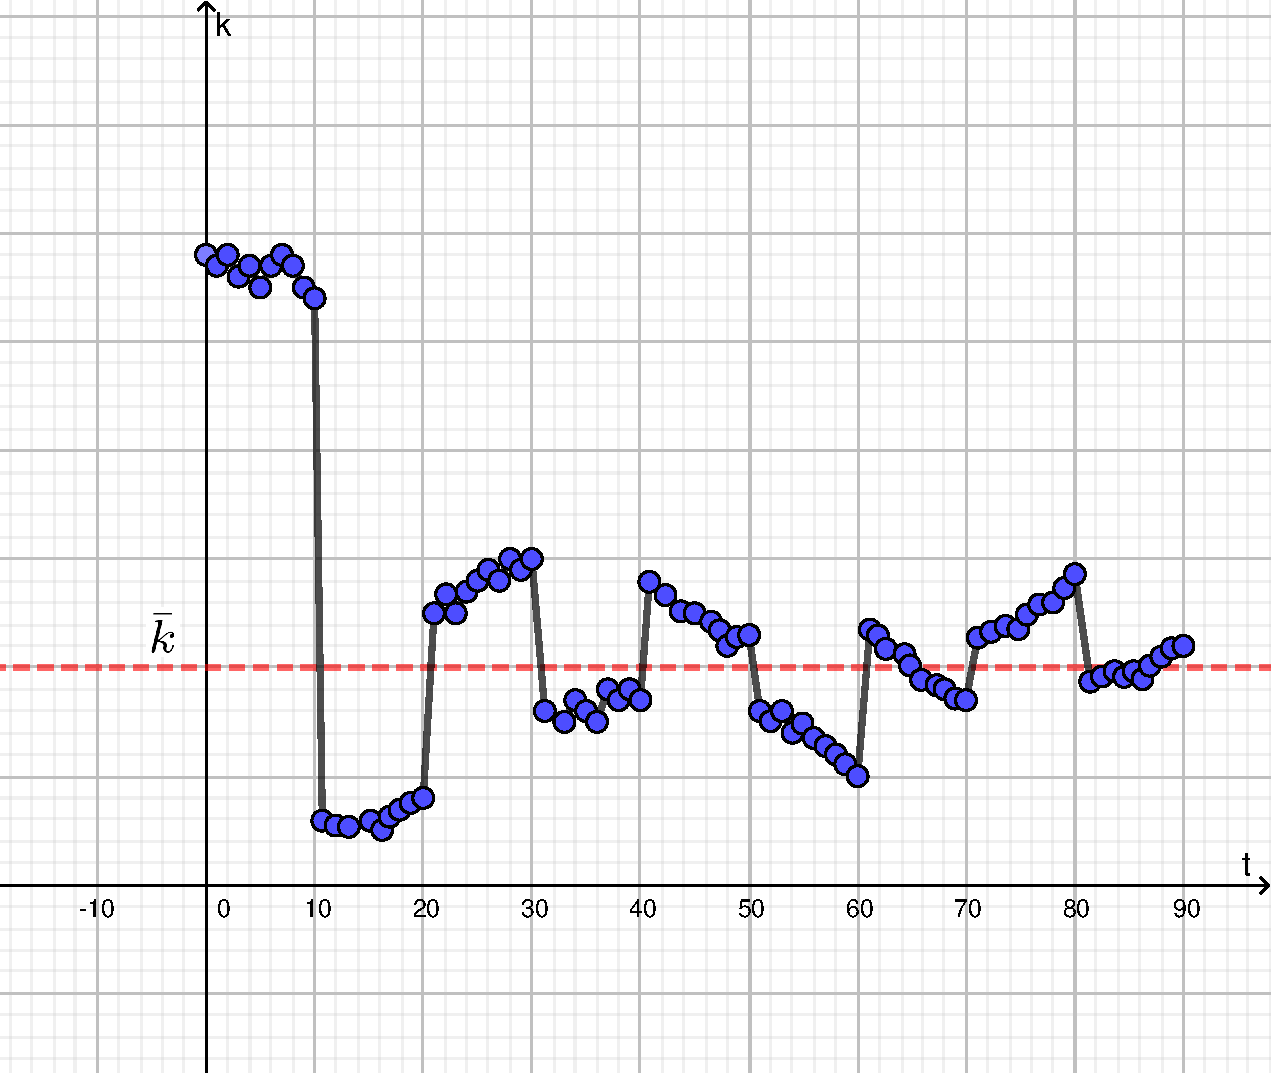
\includegraphics[width=0.7\textwidth]{Thermostats/images/thermalization.pdf}
  \caption{Thermalization of a system generated by the Andersen thermostat.\\
  Here each individual atom is separately randomized and at every 10 steps, the kinetic energy is indirectly controlled by the randomization of the velocity, which forces it to get a value which is found somewhere around $\Bar{K}$ (red dashed line). To be more accurate, this value is chosen randomly from a central $\chi ^2$ distribution with n degrees of freedom \cite{Chi-squared} (a special case of the $\Gamma$ distribution, with $K=n/2$ and $\theta=2$), which is the distribution resulting from the sum of squares of Gaussian distributed numbers, with zero mean).
  \hspace{\textwidth}}
  \label{Fig:thermalization}
\end{figure}

The choice of the stride,  (that is the only parameter here, corresponding to the $\tau$ in Berendsen), is quite significant: it affects the efficiency of the system, since it determines how frequently we apply the thermostat. In particular, when it is small, the kinetic energy of the individual atoms will relax around $\Bar{K}$ faster, but the algorithm gets slower, while when it is big, the properties of the system are more realistic, because we have smaller perturbations on the original dynamics, obtained with Hamilton equations.

Some important properties of Andersen algorithm can be listed as:\\
$+$ canonical distribution\\
$-$ not a differential equation\\
$\pm$ equilibrates well: this is a tricky point (very heuristic, system dependent), because by randomizing each atom's velocity with a too short stride, instead of equilibrating faster we slow down the dynamics of the system and we obtain the opposite thing. This happens because, even though the kinetic energy changes very quickly, the atoms move slower: the obstacles to the atomic motions will not be the collisions with other atoms, but the "collisions with the thermal bath" (so the randomization of the velocities that we performed).
\\

There are other possible ways of implementing the Andersen thermostat, which are explained in the original paper (see \cite{Andersen}). Instead of randomizing all the atom velocities every 10 steps, what can be done is to randomize at every step the velocity of one of the atoms picked at random (a small variation of this, but a very complicated one, is to pick a set of atoms at each step, making sure we don't pick again the same set of atoms). In essence, there are many ways to perform this randomization of particle velocities, and the one explained here is probably the most simple and more used, but anyway it's possible to map between one and the other.

\subsection{Langevin thermostat (1978)}

We now want to transform the Andersen thermostat which is discrete in time, to something continuous. 
To make a mental picture of what we do, remember what was done for the Berendsen thermostat: instead of forcing the system to go directly to $\Bar{K}$, as we did with velocity rescaling, with Berendsen we go to some average between $\Bar{K}$ and the current value of the kinetic energy. Here, instead of going directly to the random number that we draw, as we did with Andersen thermostat, we go to some average between the random number and the current value of the velocity.
To do so, we modify Andersen algorithm in this way (assuming we are in 1D):

 \begin{algorithm}[H]\label{Langevin_algorithm}
			\caption{Langevin algorithm}
			\begin{algorithmic}[1]
				\For{$i=1,...,nsteps$}
				\State $p=p+f*\Delta t/2$
				\State $q=q+p*\Delta t/m$
				\State $p=p+f*\Delta t/2$
				\State $p=c_1*p+c_2*\sqrt{mk_BT}*normal()$
				\EndFor
			\end{algorithmic}
\end{algorithm}
		
Let's see what happens with some choices of the parameters $c_1$ and $c_2$ :
\begin{itemize}
\item With $c_1=1$ and $c_2=0$ \hspace{0.5cm} $\Longrightarrow$ \hspace{0.5cm} No thermostat
\item With $c_1=0$ and $c_2=1$ \hspace{0.5cm} $\Longrightarrow$ \hspace{0.5cm} Andersen thermostat, applied at every step
\item With $c_1=e^{-\frac{\Delta t}{\tau}}$ and $c_2= \sqrt{1- e^{-\frac{2\Delta t}{\tau}}}$ \hspace{0.5cm} $\Longrightarrow$ \hspace{0.5cm} Langevin thermostat
\end{itemize}
In order to choose the values of $c_1$ and $c_2$ we make this observation: the term multiplied to $c_2$ is a Gaussian random number (with zero mean and variance equal to $mk_B T$), and also the $p$ to which $c_1$ is multiplied is distributed according to the canonical distribution (a Gaussian with zero mean and variance equal to $mk_B T$). Since we want balance, we need to make sure that the resulting p (on the l.h.s.) is also canonically distributed (with $\mathbb{E}(p)=0$ and $\mathbb{V}ar(p)=mk_BT$ ), so we must impose that  
$c_1^2+c_2^2 = 1$. More formally:

    \begin{align*}
    \mathbb{V}ar(p) &= \mathbb{V}ar(c_1*p+c_2*\sqrt{mk_BT}*normal()) =\\
                    &= \mathbb{V}ar (c_1*p) + \mathbb{V}ar(c_2*\sqrt{mk_BT}*normal())=\\
                    &= c_1^2*\mathbb{V}ar (p) + c_2^2*\mathbb{V}ar(\sqrt{mk_BT}*normal())=\\
                    &= c_1^2*mk_BT + c_2^2*mk_BT=\\
                    &= (c_1^2+ c_2^2)*mk_BT
    \end{align*}

As we did for the Berendsen thermostat, we take the limit to an infinitesimal time-step in order to see which is the resulting differential equation:

\begin{align*}
p(t+\Delta t) \hspace{0.3cm}&=\hspace{0.3cm} c_1*p(t) + c_2*\sqrt{mk_BT}*\boldsymbol{R}(t) =\\
&=\hspace{0.3cm} e^{-\frac{\Delta t}{\tau}}*p(t) + \sqrt{(1- e^{-\frac{2\Delta t}{\tau}})*mk_BT}*\boldsymbol{R}(t) \\ \\
\implies \lim_{\Delta t\to 0} p(t+\Delta t) \hspace{0.3cm} &=\hspace{0.3cm} \left(1-\frac{\Delta t}{\tau}\right)*p(t) +\sqrt{mk_BT\left(1-1+\frac{2\Delta t}{\tau}\right)}*\boldsymbol{R}(t) \\
\implies \lim_{\Delta t\to 0} p(t+\Delta t)-p(t) \hspace{0.3cm}&= \hspace{0.3cm} -\frac{\Delta t}{\tau}*p(t) +\sqrt{mk_BT*\frac{2\Delta t}{\tau}}*\boldsymbol{R}(t) \\ \\
\implies \Delta p \hspace{0.3cm}&=\hspace{0.3cm} -\gamma p \Delta t +\sqrt{2mk_BT\gamma}*\boldsymbol{\Delta w}(t)\\
&\big\downarrow \lim_{\Delta t\to 0} \hspace{0.15cm},\hspace{0.15cm} \textrm{many particles}\\
\implies \delta p_i \hspace{0.3cm}&=\hspace{0.3cm} -\gamma p_i \delta t +\sqrt{2m_ik_BT\gamma}*\boldsymbol{\delta w_i}(t)\\
\end{align*}

Where $\boldsymbol{R}(t)$ is a Gaussian random number $\left(P(\boldsymbol{R}(t)) \propto e^{-\frac{\boldsymbol{R}(t)^2}{2}}\right)$, which was replaced by another random factor : $\boldsymbol{\delta w}(t) = \sqrt{\Delta t}*\boldsymbol{R}(t)$. The change of variable $\tau = \frac{1}{\gamma}$ is quite relevant since it brings up a new parameter, $\gamma$, called friction. The choice of its name becomes clear if we look at the first factor of the last equation, which we call the \textit{friction factor}. Here $\gamma$ has the dimensions of $\frac{force}{momentum}$, and it acts in the direction opposite to the one of the velocity of the particle, so the physical effect of this parameter is to slow down the particle.
The second factor of the last equation is what we call \textit{stochastic factor}, and it represents the noise deriving from a temperature different from zero.

The last equation that we obtained is a stochastic differential equation and it is called Langevin equation. If our system is at equilibrium, then the temperature is the same for every particle, and the random number is independent for every degree of freedom of the system. 
In most of the cases it's more suitable and effective to use the same friction for all the particles, which will tell us, irrespectively of the mass of the particles, how quickly they will thermalize. Though, there are some situations where it's better to make $\gamma$ "particle dependent": for example when studying the dynamical properties of proteins we could decide to fix $\gamma =0$ on the protein atoms and $\gamma = 1 ps^{-1}$ on the water atoms, so that the trajectory of the proteins is perturbed less, and our dynamics is more realistic. 

Using the differential formalism (Ito convention), the underdamped Langevin equations are:
\begin{equation}
    \begin{cases}
    dq = \color{blue}{\frac{p}{m}dt}\\
    dp = \color{blue}{f dt} \color{red}{-\gamma p dt + \sqrt{2mK_BT\gamma}* \boldsymbol{\delta w}}
    \end{cases}
\end{equation}

We can think of them as a combination of two blocks: the Hamilton equations, in \textcolor{blue}{blue}, and the Langevin equation for the velocity, in \textcolor{red}{red}.

It's possible to perform the Trotter splitting (see eq. \ref{eq_trotter_splitting}) on the Langevin algorithm:

\begin{algorithm}[H]\label{Langevin_trotter}
			\caption{Langevin with Trotter splitting}
			\begin{algorithmic}[1]
			    \For{$i=1,...,nsteps$}
				\State $p=e^{-\frac{\gamma \Delta t}{2}}p + \sqrt{mk_BT \left(1-e^{-\frac{2\gamma \Delta t}{2}}\right)}*\boldsymbol{R}$
				\State $p=p+f*\Delta t/2$
				\State $q=q+p*\Delta t/m$
				\State $p=p+f*\Delta t/2$
				\State $p=e^{-\frac{\gamma \Delta t}{2}}p + \sqrt{mk_BT \left(1-e^{-\frac{2\gamma \Delta t}{2}}\right)}*\boldsymbol{R}$
				\EndFor
			\end{algorithmic}
		\end{algorithm}
		
This algorithm is the one that was given to us in SIMPLEMD (second exercise). As we saw in the chapter related to Trotter splitting, it is equivalent to write p as it was initially defined, or to duplicate the equation inside the for, and applying to them the change of time-step from $\Delta t$ to $\frac{\Delta t}{2}$. In this way, the time reversibility of the algorithm can be seen explicitly (the algorithm is symmetric), but the random numbers that are drawn here are double, which makes this version less efficient.
\\
